\chapter{Opis projektnog zadatka}
		
		\textbf{\textit{dio 1. revizije}}\\
		
		Cilj ovog projekta je razviti programsku podršku za stvaranje web aplikacije "IME APLIKACIJE". Ideja aplikacije je ponuditi običnim građanima jednostavan i efikasan način prijave oštećenja javnih površina i cesta u gradu te dobivanje povratnih informacija konkretnom oštećenju i njihovoj prijavi. 
		
		Građani će svojim djelovanjem putem aplikacije unaprjeđivati kvalitetu života u svojoj zajednici. Svojim prijavama, koje će biti javno dostupne, građani će poticati gradske urede da saniraju prijavljena oštećenja. Aplikacija će također pomoći gradskim uredima u obavljanju svojih zadaća. Naime, preko aplikacije uredi će imati puno bolji uvid u probleme koji postoje u zajednici. Zahvaljujući aplikaciji uredi će moći brže i kvalitetnije reagirati na probleme u zajednici.
		
		Građani koriste web aplikaciju u anonimnom načinu, to jest ne prijavljuju se u sustav. Na naslovnoj stranici korisniku građaninu ponuđene su opcije podnošenja nove prijave, pregleda postojećih prijava i pregled statistike prijava.
		
		Korisniku se prilikom odabira podnošenja nove prijave otvara obrazac koji je potrebno ispuniti. Prijava sadrži naslov koji definira oštećenje. Slijedi kratak opis u kojem korisnik detaljnije opisuje oštećenje u slobodnoj formi. Korisnik dalje prilaže geografski položaj oštećenja koje se prijavljuje. Geografski položaj se definira odabirom položaja na karti koja će se moći otvoriti prilikom ispunjavanja obrasca ili upisivanjem adrese na kojoj se nalazi oštećenje. Također korisnik će moći priložiti geografski položaj automatski preko svoje trenutne lokacije. Korisniku se nudi opcija da uz prijavu priloži fotografije oštećenja. Ukoliko korisnik priloži fotografije, aplikacija će pokušati iz njih izvući podatke o lokaciji te ih ponuditi korisniku kao lokaciju oštećenja. Korisnik u prijavi mora odabrati gradski ured nadležan za konkretan problem. Prilikom opisivanja oštećenja aplikacija će pokušati sama zaključiti koji ured bi mogao biti nadležan za problem koji se prijavljuje te će isti predložiti korisniku. Također, ako u sustavu već postoji slična nedavna prijava na istoj lokaciji aplikacija će predložiti korisniku već postojeću prijavu i ponuditi mu da svoju prijavu nadoveže na već postojeću. Korisnik u prijavi može ostaviti mail na koji želi dobivati obavijesti o statusu njegove prijave. Nakon podnošenja prijave aplikacija korisniku daje jedinstveni kod podnesene prijave koja služi za praćenje te prijave preko same aplikacije.
		
		Prilikom odabira pregleda postojećih prijava korisniku se otvara lista svih aktivnih prijava. Lista se može filtrirati po vremenu podnošenja prijave, lokaciji, statusu, nadležnom gradskom uredu, vrsti oštećenja i slično. Korisnik također može pretraživati prijave po jedinstvenom kodu prijave. Na taj način svaki korisnik može pregledavati svoje prijave na aplikaciji. Za svaku prijavu se prikazuju informacije iz podnesenog obrasca. Također se prikazuje status prijave (na čekanju, rješava se, riješena), broj prijava koje su vezane za ovu prijavu, odnosno prijava za koju je vezana ova prijava. Prijave sa riješenim statusom su korisniku dostupne jedino preko odgovarajućeg koda prijave. Pregled prijava je također moguć preko karte.
		
		Prikaz statistike prijava nudi filtriranje podataka po lokaciji prijave, vremenu podnošenja prijave, uredu i vrsti oštećenja. Za odabrane parametre aplikacija prikazuje:
		\begin{packed_item}
			\item ukupan broj podnešenih prijava
			\item broj prijava koje su na čekanju i njihov udio
			\item broj prijava koje su u procesu rješavanja i njihov udio
			\item broj prijava koje su riješene i njihov udio
			\item prosječan broj podnesenih prijava u danu
			\item prosječan broj dana koji prijava provede na čekanju
			\item prosječan broj dana za vrijeme kojih je prijava u procesu rješavanja
		\end{packed_item}
		
		
		---------------------
		
		
		
		\textit{Na osnovi projektnog zadatka detaljno opisati korisničke zahtjeve. Što jasnije opisati cilj projektnog zadatka, razraditi problematiku zadatka, dodati nove aspekte problema i potencijalnih rješenja. Očekuje se minimalno 3, a poželjno 4-5 stranica opisa.	Teme koje treba dodatno razraditi u ovom poglavlju su:}
		\begin{packed_item}
			\item \textit{potencijalna korist ovog projekta}
			\item \textit{postojeća slična rješenja (istražiti i ukratko opisati razlike u odnosu na zadani zadatak). Dodajte slike koja predočavaju slična rješenja.}
			\item \textit{skup korisnika koji bi mogao biti zainteresiran za ostvareno rješenje.}
			\item \textit{mogućnost prilagodbe rješenja }
			\item \textit{opseg projektnog zadatka}
			\item \textit{moguće nadogradnje projektnog zadatka}
		\end{packed_item}
		
		\textit{Za pomoć pogledati reference navedene u poglavlju „Popis literature“, a po potrebi konzultirati sadržaj na internetu koji nudi dobre smjernice u tom pogledu.}
		\eject
		
		\section{Primjeri u \LaTeX u}
		
		\textit{Ovo potpoglavlje izbrisati.}\\

		U nastavku se nalaze različiti primjeri kako koristiti osnovne funkcionalnosti \LaTeX a koje su potrebne za izradu dokumentacije. Za dodatnu pomoć obratiti se asistentu na projektu ili potražiti upute na sljedećim web sjedištima:
		\begin{itemize}
			\item Upute za izradu diplomskog rada u \LaTeX u - \url{https://www.fer.unizg.hr/_download/repository/LaTeX-upute.pdf}
			\item \LaTeX\ projekt - \url{https://www.latex-project.org/help/}
			\item StackExchange za Tex - \url{https://tex.stackexchange.com/}\\
		
		\end{itemize} 	


		
		\noindent \underbar{podcrtani tekst}, \textbf{podebljani tekst}, 	\textit{nagnuti tekst}\\
		\noindent \normalsize primjer \large primjer \Large primjer \LARGE {primjer} \huge {primjer} \Huge primjer \normalsize
				
		\begin{packed_item}
			
			\item  primjer
			\item  primjer
			\item  primjer
			\item[] \begin{packed_enum}
				\item primjer
				\item[] \begin{packed_enum}
					\item[1.a] primjer
					\item[b] primjer
				\end{packed_enum}
				\item primjer
			\end{packed_enum}
			
		\end{packed_item}
		
		\noindent primjer url-a: \url{https://www.fer.unizg.hr/predmet/proinz/projekt}
		
		\noindent posebni znakovi: \# \$ \% \& \{ \} \_ 
		$|$ $<$ $>$ 
		\^{} 
		\~{} 
		$\backslash$ 
		
		
		\begin{longtblr}[
			label=none,
			entry=none
			]{
				width = \textwidth,
				colspec={|X[8,l]|X[8, l]|X[16, l]|}, 
				rowhead = 1,
			} %definicija širine tablice, širine stupaca, poravnanje i broja redaka naslova tablice
			\hline \SetCell[c=3]{c}{\textbf{naslov unutar tablice}}	 \\ \hline[3pt]
			\SetCell{LightGreen}IDKorisnik & INT	&  	Lorem ipsum dolor sit amet, consectetur adipiscing elit, sed do eiusmod  	\\ \hline
			korisnickoIme	& VARCHAR &   	\\ \hline 
			email & VARCHAR &   \\ \hline 
			ime & VARCHAR	&  		\\ \hline 
			\SetCell{LightBlue} primjer	& VARCHAR &   	\\ \hline 
		\end{longtblr}
		

		\begin{longtblr}[
				caption = {Naslov s referencom izvan tablice},
				entry = {Short Caption},
			]{
				width = \textwidth, 
				colspec = {|X[8,l]|X[8,l]|X[16,l]|}, 
				rowhead = 1,
			}
			\hline
			\SetCell{LightGreen}IDKorisnik & INT	&  	Lorem ipsum dolor sit amet, consectetur adipiscing elit, sed do eiusmod  	\\ \hline
			korisnickoIme	& VARCHAR &   	\\ \hline 
			email & VARCHAR &   \\ \hline 
			ime & VARCHAR	&  		\\ \hline 
			\SetCell{LightBlue} primjer	& VARCHAR &   	\\ \hline 
		\end{longtblr}
	


		
		
		%unos slike
		\begin{figure}[H]
			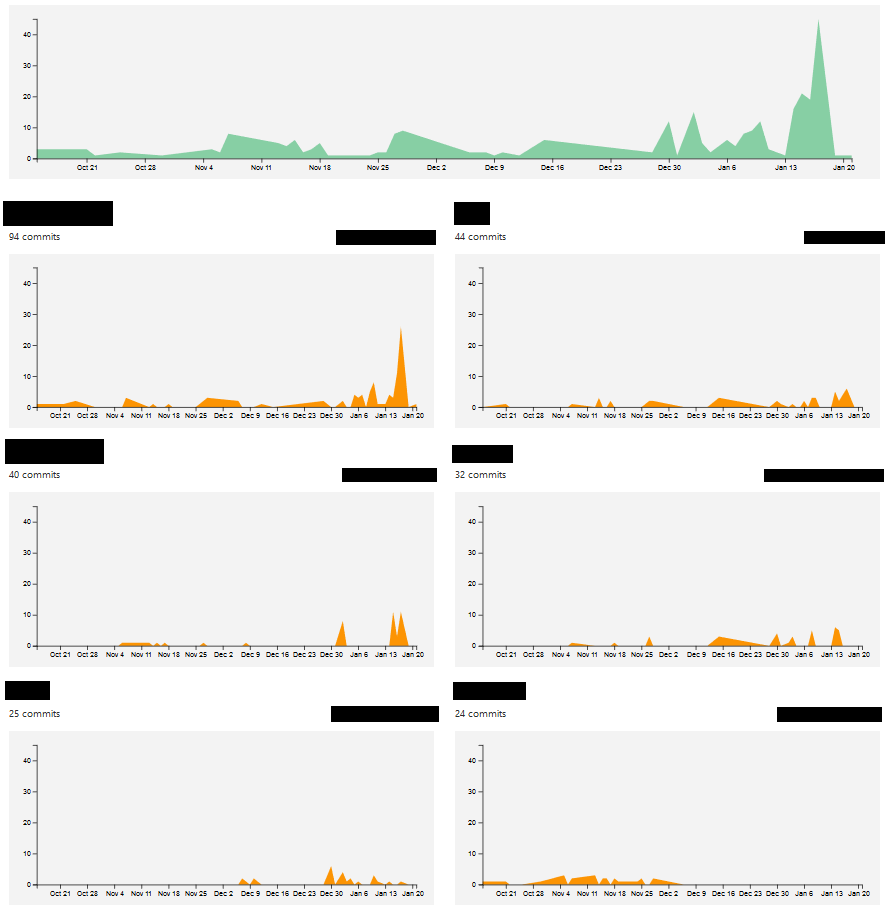
\includegraphics[scale=0.4]{slike/aktivnost.PNG} %veličina slike u odnosu na originalnu datoteku i pozicija slike
			\centering
			\caption{Primjer slike s potpisom}
			\label{fig:promjene}
		\end{figure}
		
		\begin{figure}[H]
			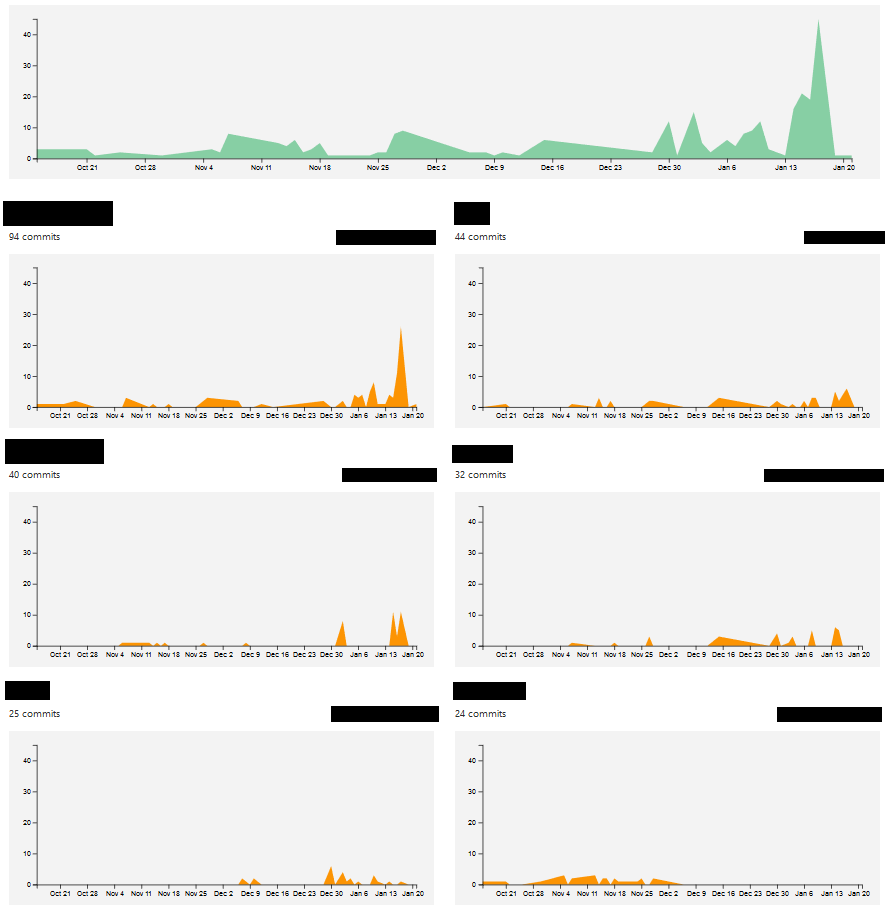
\includegraphics[width=\textwidth]{slike/aktivnost.PNG} %veličina u odnosu na širinu linije
			\caption{Primjer slike s potpisom 2}
			\label{fig:promjene2} %label mora biti drugaciji za svaku sliku
		\end{figure}
		
		Referenciranje slike \ref{fig:promjene2} u tekstu.
		
		\eject
		
	